% !TEX root = ../beamer.tex

\begin{frame}[fragile, plain]
	\plainnumber
	\frametitle{Workflow Specification}
	
	\begin{minipage}{0.45\textwidth}
	    		        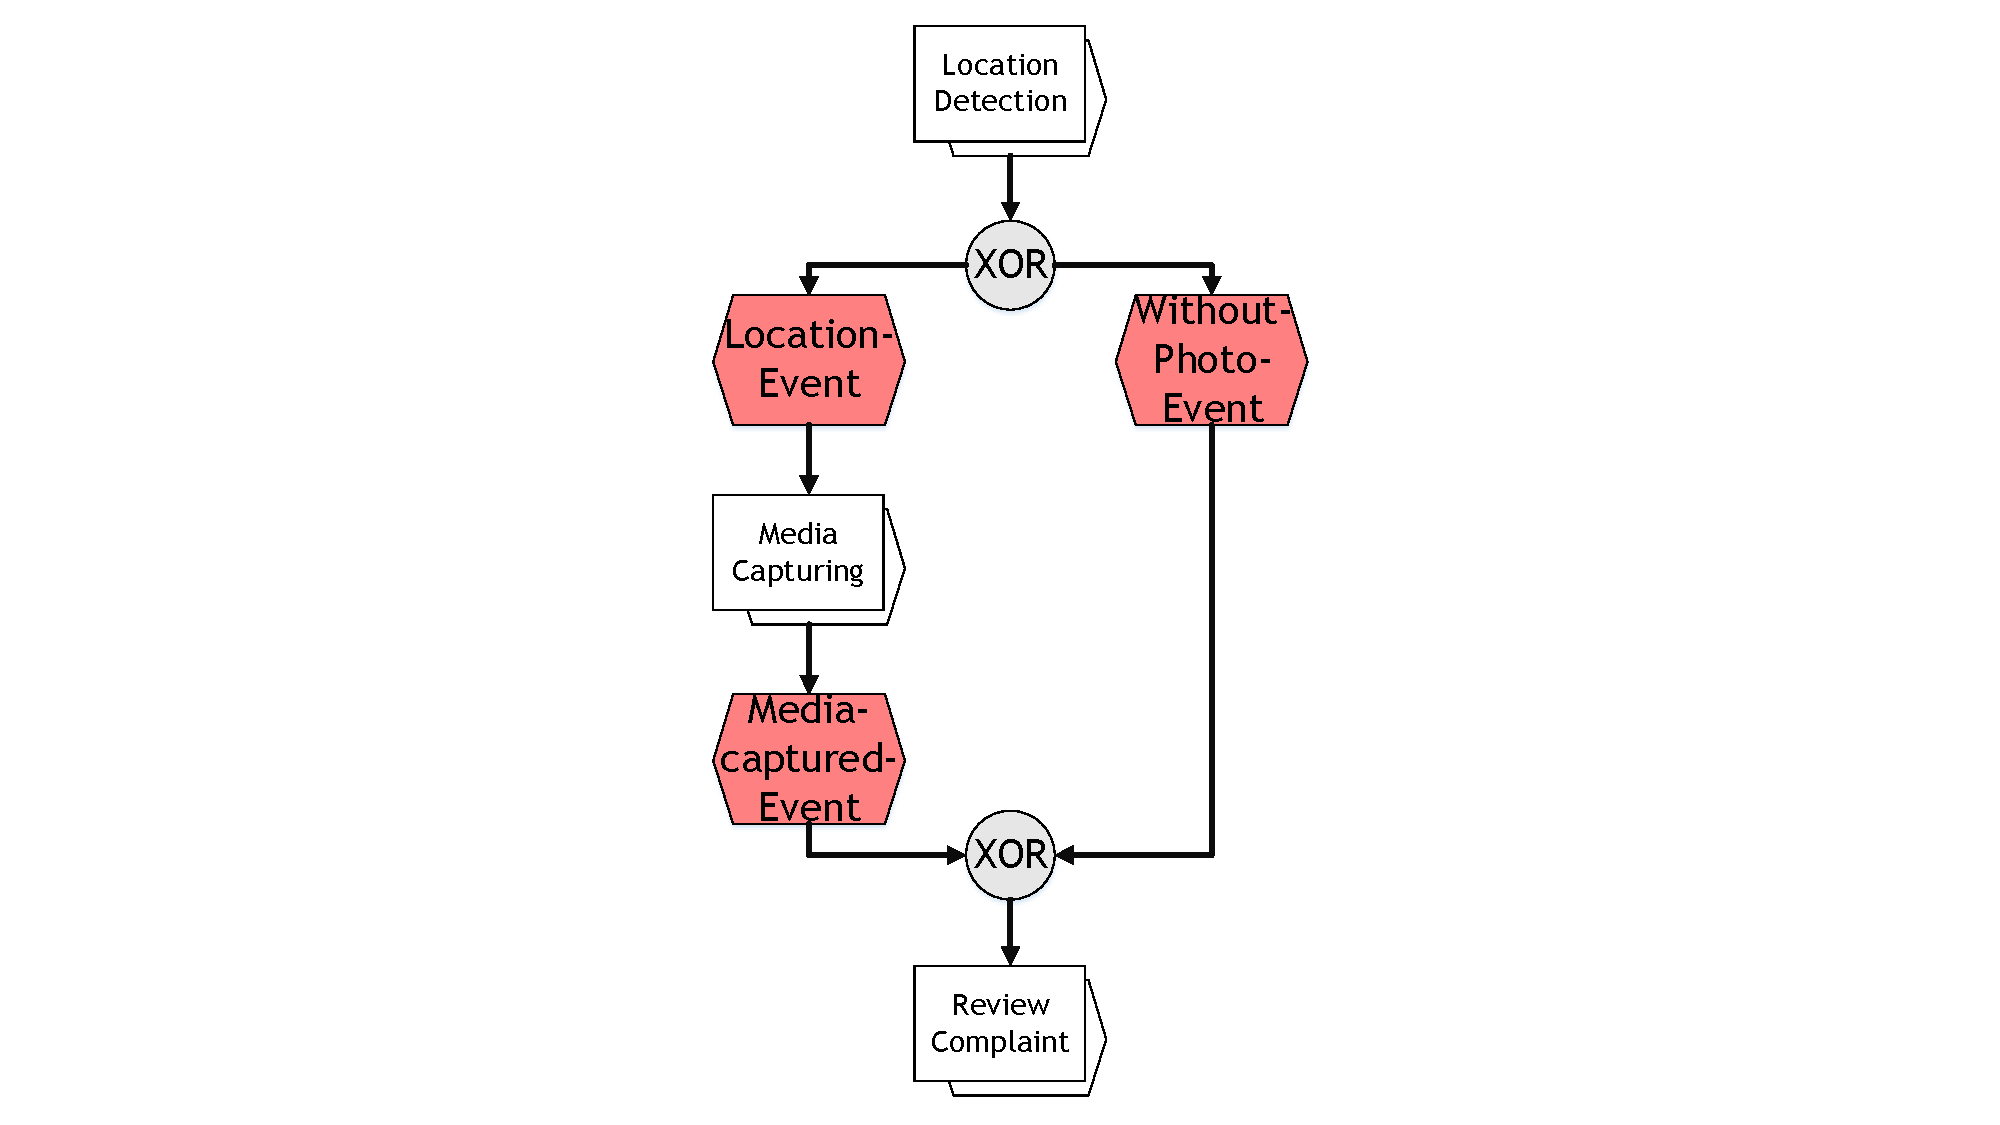
\includegraphics[height = 7cm, trim = 10cm 0cm 10cm 0cm, clip = true]{images/WorkflowSpecification.pdf}	  
	\end{minipage}\hfill
	\begin{minipage}{0.5\textwidth}
\begin{lstlisting}
WorkflowElement LocationDetection
  fires LocationEvent {
    start Mediacapturing
  }
  fires WithoutPhotoEvent {
    start ReviewComplaint
  }

WorkflowElement MediaCapturing
  fires MediacapturedEvent {
    start ReviewComplaint
  }

WorkflowElement ReviewComplaint
  fires EndEvent {
    end workflow
  }
\end{lstlisting}
\end{minipage}

\end{frame}

%-----------------------------------------------------------------------------------

\begin{frame}[fragile, plain]
	\plainnumber
	\frametitle{Workflow Specification Across Apps}
	
	\begin{minipage}{0.45\textwidth}
	    		        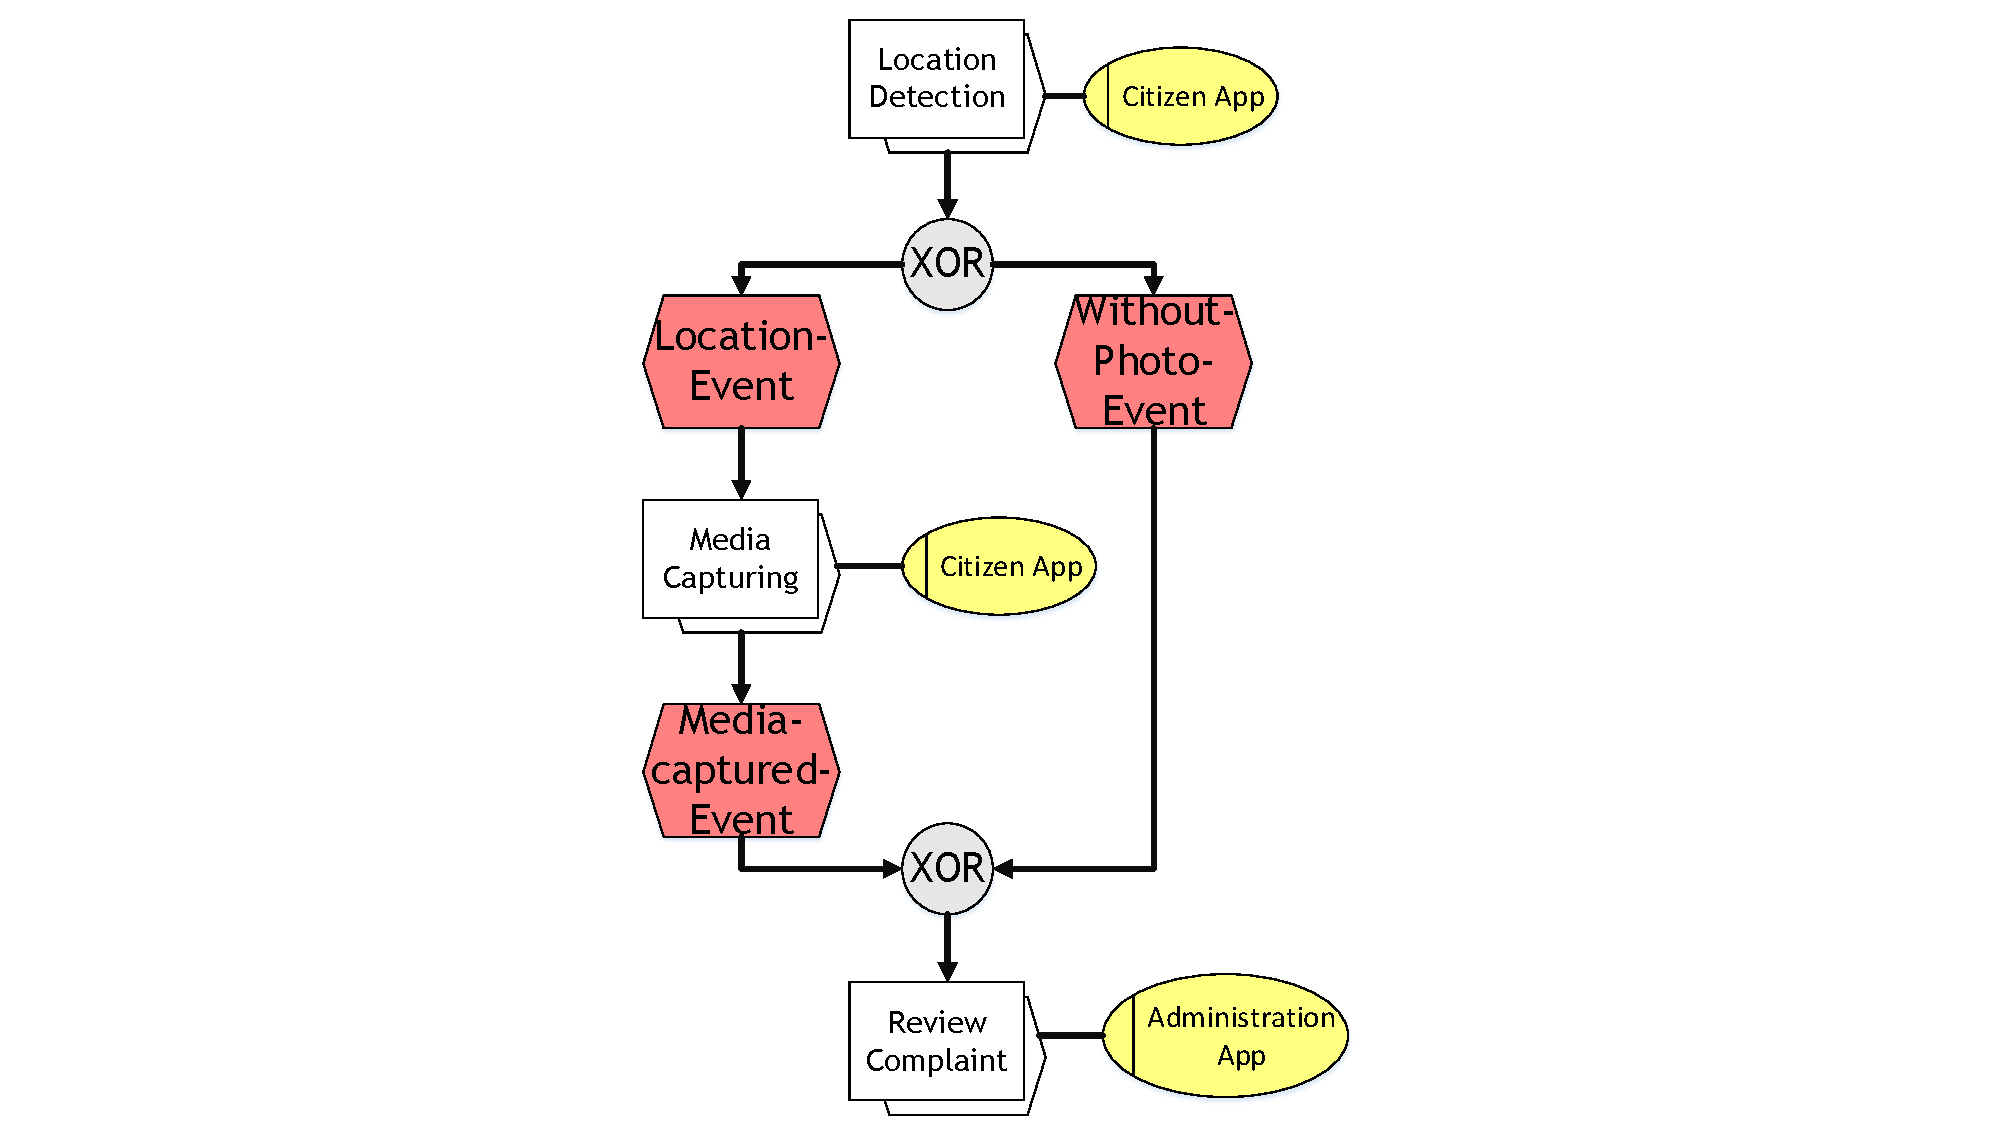
\includegraphics[height = 7cm, trim = 10cm 0cm 10cm 0cm, clip = true]{images/wfAcrossApps}	  
	\end{minipage}\hfill
	\begin{minipage}{0.5\textwidth}
\begin{lstlisting}
App CitizenApp {
  WorkflowElements {
    LocationDetection (startable: "Start Complaint"),
    MediaCapturing
  }
}

App AdministrationApp {
  WorkflowElements {
    ReviewComplaint
  }
}
\end{lstlisting}
\end{minipage}

\end{frame}


\begin{frame}[fragile]
	\frametitle{Calling External Webservices}
\begin{lstlisting}[basicstyle=\footnotesize\ttfamily]
externalWebService sendEmail {
  url "http://psmd2.uni-muenster.de:8080/SendMail/api/mail/send/"
   method GET
   queryparams (
     "to" : "md2@trashmail.de"
     "subject" : "Map.Apps E-Mail"
     "body" : "Dear ladies and gentlemen, this is an e-mail sent by md2 map.apps!"
   )
}
	
bind action WebServiceCall sendEmail on EmailView.SendButton.onClick
\end{lstlisting}
\end{frame}

\begin{frame}[fragile]
	\frametitle{Starting Workflows from External WS Calls}
\begin{lstlisting}[basicstyle=\footnotesize\ttfamily]
WorkflowElement LocationDetection (invokable)
  fires ...
		
invokable at "address" using POST {
  set :ComplaintProvider.loc to :AddressProvider
  :AddressProvider.myStreet
  :AddressProvider.myStreetNo
  :AddressProvider.myCity
  :AddressProvider.myPostalCode
  default :ComplaintProvider.status = "User is filling out complaint" 
}
\end{lstlisting}
\end{frame}



%-----------------------------------------------------------------------------------

\begin{frame}[plain]

\plainnumber

\frametitle{Implementation: WorkflowEventHandler}

\begin{center}
	\begin{tikzpicture}[
	>=stealth,
	wfe/.style = {draw, circle, fill=black!15!white},
	eh/.style = {draw, minimum height = 3cm, minimum width = 3cm, fill=pantone315!30!white}
	]
		\node (citizen) {
\includegraphics[width=0.5cm]{images/stickfigure}};
		\node[below = 0cm of citizen] (citizenlbl) {\scriptsize Citizen};
		
		\node[wfe, below = of citizenlbl] (wfe1) {WFE1};
		\node[wfe, below = of wfe1] (wfe2) {WFE2};
		\node[eh, right = 2cm of wfe1.north east, anchor = north west] (eh) {Event Handler};
		\node[draw, minimum width = 2cm, minimum height = 1cm, right = 2cm of eh, fill=pantone369!20!white] (be) {Backend};
		
		\begin{pgfonlayer}{bg}
			\draw[fill=pantone396!10!white, draw=pantone396] ($ (wfe1.north west) + (-0.4, 0.4) $) rectangle  ($ (eh.south east) + (0.5, -0.5) $);
		\end{pgfonlayer}
		
		\draw<1->[->, thick] (citizenlbl) -- node[right] {\scriptsize{\texttt{start}}} (wfe1);
		\draw<2->[->, thick] (wfe1) -- node[above, sloped] {\scriptsize{\texttt{ID, event}}} (eh);
		\draw<3->[->, thick] (eh.west) -- node[above, sloped] {\scriptsize{\texttt{changeWFE}}} (wfe2.north east);
		\draw<4->[->, thick] (wfe2.east) -- node[below, sloped] {\scriptsize{\texttt{ID, event}}} (eh);
		\draw<5->[->, thick] (eh) -- node[above] {\scriptsize{\texttt{ID, event}}} (be);
		
		\visible<6->{
			\node[above right = 0.75cm and 1.5cm of citizenlbl] (admin) {
\includegraphics[width=0.5cm]{images/stickfigure}};
			\node[below = 0cm of admin] (adminlbl) {\scriptsize Admin};
			\node[draw, fill=black!15!white, right = of admin, minimum width = 2cm, minimum height = 1cm] (looi) {LOOI};
			\draw[->, thick] (admin) -- node[above] {\scriptsize{\texttt{show}}} (looi);
		}
		\draw<7->[->, thick] ($(looi.east) + (0, 0.1) $) -| node[right] {\scriptsize{\texttt{appID}}} ($(be.north) + (0.1, 0)$);
		\draw<8->[<-, thick] ($(looi.east) + (0, -0.1) $) -| node[below left] {\scriptsize{\texttt{open issues}}} ($(be.north) + (-0.1, 0)$);
		\visible<9->{
			\node[wfe, below right = 0.5cm of looi] (wfe3) {WFE3};
			\draw[->, thick] (looi) |- node[above right] {\scriptsize{\texttt{start}}} (wfe3);	
		}
			\begin{pgfonlayer}{bg}
				\draw<6->[fill=pantone396!10!white, draw=pantone396] ($ (looi.north west) + (-0.4, 0.4) $) rectangle  ($ (wfe3.south east) + (0.5, -0.5) $);
			\end{pgfonlayer}
		
	\end{tikzpicture}
\end{center}

\end{frame}


\begin{frame}
    \frametitle{DSL}
\end{frame}

\begin{frame}
    \frametitle{Generated Code}
\end{frame}

%\begin{frame}
%    \frametitle{Generator}
%    
%	\begin{center}   
%	\begin{tikzpicture}[
%		>=stealth,
%		node distance = 0.75cm and 0.25cm,
%		every node/.style={minimum height = 1.75em}]
%		\node[draw] (dsl) {DSL\vphantom{Aq}};
%		\node[draw, below = of dsl] (md2model) {\MD Model\vphantom{Aq}};
%		\draw[->] (md2model) -- node[right] {\tiny{uses}} (dsl);
%	    
%		\node[below = of md2model, draw] (preprocessor) {Preprocessor\vphantom{Aq}};
%		\draw[->] (md2model) -- node[right] {\tiny{processed by}} (preprocessor);
%		
%		\node[draw, below = of preprocessor] (generator) {Generator\vphantom{Aq}};
%		
%		\draw[->] (preprocessor) -- node[right] {\tiny{input for}} (generator);
%		
%		\node[draw, below left = 0.25cm of generator] (mapapps) {map.apps source\vphantom{Aq}};
%		\node[draw, below right = 0.25cm of generator] (backend) {backend source\vphantom{Aq}};
%		
%		\draw[->] (generator) -| node[above] {\tiny{generates}} (mapapps);
%		\draw[->] (generator) -| node[above] {\tiny{generates}} (backend);
%	\end{tikzpicture}
%	\end{center}
%\end{frame}

\begin{frame}
    \frametitle{Deployment}
    
    \begin{center}   
	    \begin{tikzpicture}[
	    >=stealth,
	    node distance = 0.75cm and 0.25cm,
	    big/.style = {draw, minimum width = 2.5cm, minimum height = 1.75em}
	    ]
	    \node[big] (generator) {Generator};
	    \node[big, below left = of generator] (mapapps) {map.apps source\vphantom{Aq}};
	    \node[big, below right = of generator] (backend) {backend source\vphantom{Aq}};
	    \draw[->] (generator) -| node[above] {\tiny{generates}} (mapapps);
	    \draw[->] (generator) -| node[above] {\tiny{generates}} (backend);
	    \node[big, rounded corners, below = of mapapps] (jetty) {Jetty\vphantom{Aq}};
	    \node[big, rounded corners, below = of backend] (glassfish) {Glassfish\vphantom{Aq}};
	    \draw[->] (mapapps) -- node[left] {\tiny{deployed on}} (jetty);
	    \draw[->] (backend) -- node[right] {\tiny{deployed on}} (glassfish);
	    \draw[<->] (jetty) -- node[above] (communicates) {\tiny{communicates}} (glassfish);
	    
	    \node[big, rounded corners, below = of communicates] (tomcat) {Tomcat};
	    \node[big, gray, below = 0cm of tomcat] {map.apps full};	    
	    
	    \end{tikzpicture}
    \end{center}
\end{frame}


\begin{frame}
    \frametitle{Modeling, Generation \& Deployment}
    
    \begin{center}   
	    \begin{tikzpicture}[
	    >=stealth,
	    node distance = 0.75cm and 0.25cm,
	    big/.style = {draw, minimum width = 2.5cm, minimum height = 1.75em}
	    ]
	    \node[big, fill=pantone315!30!white] (eclipseDevelopment) {Eclipse Development IDE};
	    \node[big, below = 0.05cm of eclipseDevelopment] (dsl) {DSL};
	    \node[big, below = 0.05cm of dsl] (generator) {Generator};
	    
	    \node[big, below=1.4cm of generator, fill=pantone315!30!white] (generatedArtifacts) {Generated Artifacts};
	    \node[big, below = 0.05cm of generatedArtifacts] (backend) {backend};
	    \node[big, below = 0.05cm of backend] (mapApps) {map.apps};
	    
	    \node[big, right = 2cm of backend] (wildfly) {Wildfly AS};
	    \node[big, right = 2cm of mapApps] (jetty) {Jetty};
	    
	    \draw[->] (backend) -- node[above] {\tiny{deploy}} (wildfly);
	    \draw[->] (mapApps) -- node[above] {\tiny{deploy}} (jetty);
	    
	    \node[big, right = 2cm of eclipseDevelopment, fill=pantone315!30!white] (eclipseModeling) {Eclipse Modeling IDE};
	    \node[big, below = 0.05cm of eclipseModeling] (md2model) {\MD Model};
	    \node[below = 0cm of md2model] (modelModels) {models};
	    \node[below = 0cm of modelModels] (modelViews) {views};
	    \node[below = 0cm of modelViews] (modelController) {controllers};
	    \node[below = 0cm of modelController] (modelViews) {workflows};
	    
	    \draw[->] (md2model) -- node[above] {\tiny{uses}} (dsl);
	    \draw[->] (generator) -- node[left] {\tiny{generates}} (generatedArtifacts);
	    \draw[->] ($(eclipseModeling.south west) + (0, -1.17)$) -- node[above] {\tiny{invoces}} (generator);   

	    \draw (eclipseDevelopment.north west) rectangle ($(eclipseDevelopment.south east) + (0, -1.7)$);
	    \draw (generatedArtifacts.north west) rectangle ($(generatedArtifacts.south east) + (0, -1.7)$);
	    \draw (eclipseModeling.north west) rectangle ($(eclipseModeling.south east) + (0, -3.5)$);
	    \draw (md2model.south west) rectangle ($(md2model.south east) + (0, -2.5)$);
	    
	    
	    \end{tikzpicture}
    \end{center}
\end{frame}

\begin{frame}
    \frametitle{Deployment}
TODO: show symblinks irgendwie... oder kommt das in der live vorfuehrung?
\end{frame}

